\clearpage

\chapter{Use Case Diagramme}
Folgend wird die Software als Use Case Diagramme dargestellt. Use Cases geben die Außensicht des Systems wieder. Es werden typische Funktionalitäten beschrieben, die der Benutzer mit dem System ausführt.

%SPIELER VERWALTEN
\section{Spieler verwalten - $\backslash$LF10$\backslash$,$\backslash$LF11$\backslash$,$\backslash$LF12$\backslash$}
\begin{figure}[!h]
	\centering
    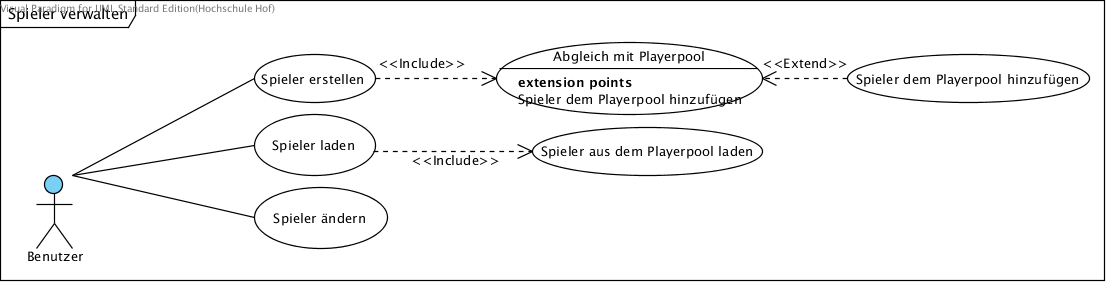
\includegraphics[width=\textwidth]{./SpielerVerwalten.png}
	\label{layout_gesamt}
\end{figure}

\subsection{Beschreibung}
\textbf{Spieler erstellen: }Der Benutzer erstellt durch die Angabe des Namens einen Spieler. Bei jeder Erstellung eines Spielers wird automatisch geprüft, ob bereits ein Spieler mit gleichem Namen existiert. Dazu wird ein Abgleich mit dem Playerpool durchgeführt.\\

\noindent \textbf{Spieler laden: }Ist der Benutzer bereits als Spieler gespeichert, kann er durch die Auswahl des Spielernamens seine Spielerdaten laden.\\

\noindent \textbf{Spieler ändern: } Gespeicherte Spieler können geändert oder gelöscht werden.\\
Bemerkung: Diese Lastenheftfunktionen wird in den weiteren Diagrammen und Ausführungen nicht weiter betrachtet, weil es letztendlich eine Kombination aus Laden und Erstellen ist und aufgrund des Umfangs nicht extra betrachtet wird.


%ANZAHL DER SPIELER
\clearpage
\section{Anzahl der Spieler wählen - $\backslash$LF20$\backslash$}
\begin{figure}[!h]
	\centering
    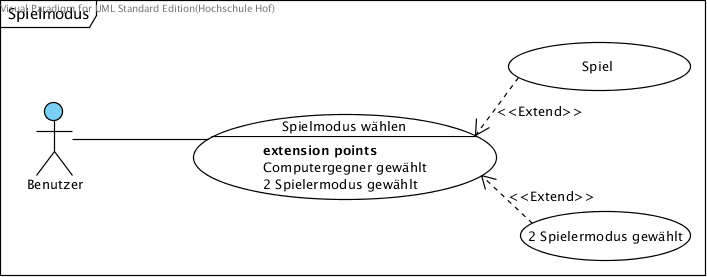
\includegraphics[width=\textwidth]{./AnzahlSpieler.png}
	\label{layout_gesamt}
\end{figure}

\subsection{Beschreibung}
\textbf{Spielmodus wählen: }Der Benutzer kann zwischen dem Modus ,,Spieler gegen Computer`` und ,,Spieler gegen Spieler`` wählen.


\vspace{2.5 cm}
%THEMA
\section{Thema wählen - $\backslash$LF30$\backslash$}
\begin{figure}[!h]
	\centering
    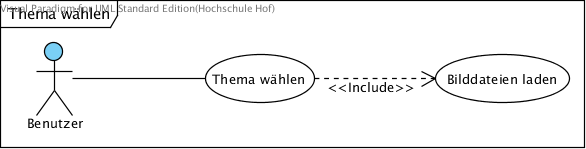
\includegraphics[width=\textwidth]{./Thema.png}
    
	\label{layout_gesamt}
\end{figure}

\subsection{Beschreibung}
\textbf{Thema wählen: }Dem Benutzer stehen die Themen ,,Tiere``, ,,Natur`` und ,,Flaggen`` zur Auswahl. Je nach gewähltem Thema werden die jeweiligen Bilddaten geladen.

%SPIELFELDGROESSE
\clearpage
\section{Spielfeldgröße wählen - $\backslash$LF40$\backslash$}
\begin{figure}[!h]
	\centering
    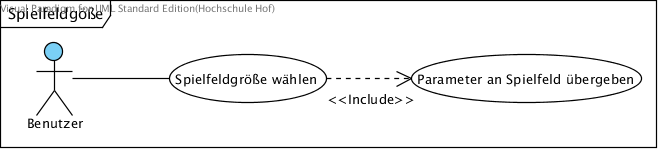
\includegraphics[width=\textwidth]{./Spielfeldgroesse.png}
	\label{layout_gesamt}
\end{figure}

\subsection{Beschreibung}
\textbf{Spielfeldgröße wählen: }Bei der Spielfeldgröße können die Größen 4x4 oder 8x8 ausgewählt werden. Anhand der Wahl wird die größe des Spielfeldes bestimmt.

%SPIEL STARTEN
\clearpage
\section{Spiel starten - $\backslash$LF50$\backslash$}
\begin{figure}[!h]
	\centering
    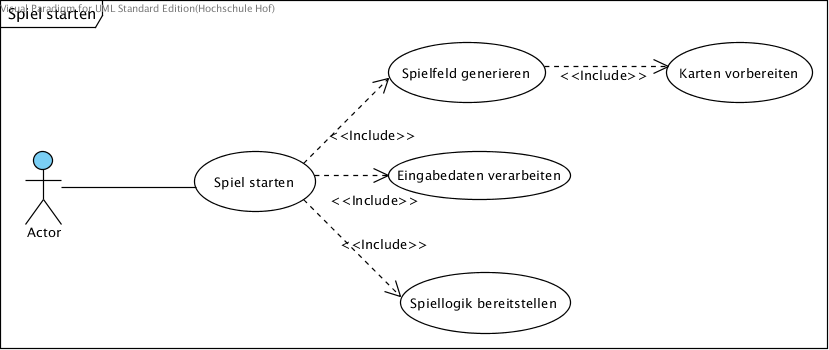
\includegraphics[width=\textwidth]{./SpielStarten.png}
	\label{layout_gesamt}
\end{figure}

\subsection{Beschreibung}
\textbf{Spiel starten: } Durch den Anwendungsfall ,,Spiel starten`` wird das Spiel gestartet. Es werden folgende Prozesse ausgelöst: Das gewünschte Spielfeld wird generiert, die Eingabedaten Name, Spielmodus, Thema werden verarbeitet und die Spiellogik wird bereitgestellt.

%HIGHSCORE
\clearpage
\section{Highscore - $\backslash$LF60$\backslash$,$\backslash$LF70$\backslash$}
\begin{figure}[!h]
	\centering
    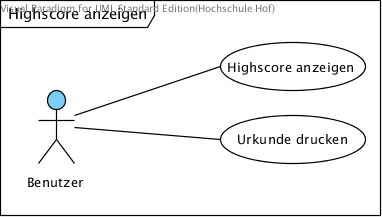
\includegraphics[width=\textwidth]{./Highscore.png}
	\label{layout_gesamt}
\end{figure}

\subsection{Beschreibung}
\textbf{Highscore anzeigen: } Der Benutzer hat die Möglichkeit, sich eine Highscore anzeigen zu lassen. Es werden die besten 10 Spieler sortiert nach erreichter Punktzahl angezeigt.\\
\textbf{Urkunde drucken: } Die Spieler aus der Highscore haben die Möglichkeit sich eine Urkunde zu drucken.

%VOKABELTRAINING
\clearpage
\section{Vokabeltraining - $\backslash$LF80$\backslash$}
\begin{figure}[!h]
	\centering
    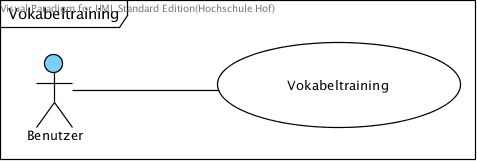
\includegraphics[width=\textwidth]{./Vokabeltraining.png}
	\label{layout_gesamt}
\end{figure}

\subsection{Beschreibung}
\textbf{Vokabeltraining: } Während des Spiels wird bei übereinstimmenden Karten das englische Equivalent zum jeweiligen Kartenmotiv abgefragt.


%AUDIODATEN
\section{Audiodaten abspielen - $\backslash$LF90$\backslash$}
\begin{figure}[!h]
	\centering
    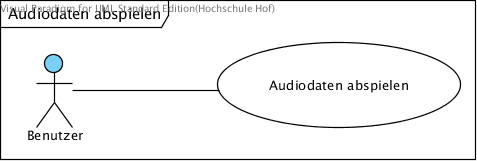
\includegraphics[width=\textwidth]{./Audiodaten.png}
	\label{layout_gesamt}
\end{figure}

\subsection{Beschreibung}
\textbf{Audiodaten abspielen: } Zum gewonnenen Kartenpaar kann ein Sound abgespielt werden. Beim Thema Tiere werden die Tierlaute wiedergegeben, bei den Flaggen die jeweilige Hymne des Landes.

